\documentclass[aspectratio=169,t]{beamer}

% Some default packages
\usepackage[english]{babel}
\usepackage[utf8]{inputenc}
\usepackage[T1]{fontenc}
\usepackage{qrcode}
\usepackage{tikz}
\usetikzlibrary{shapes.geometric}
\usepackage{pgfplots}
\usepackage{pgfplotstable}

%\pgfplotsset{compat=1.9,
	%title style={color=dlrdarkblue},
	%tick label style = {color=dlrdarkblue},
	%every axis label = {color=dlrdarkblue},
	%legend style,
	%label style = {color=dlrdarkblue}
%}
%\tikzset{cross/.style={cross out, draw=black, minimum size=2*(#1-\pgflinewidth), inner sep=0pt, outer sep=0pt},
	%default radius will be 1pt. 
	%cross/.default={1pt}}

% DLR Layout
%\usetheme[beamertools={fixblocktitle=false}, professionalfonts]{dlr}
%Select Blue, Green or Yellow as color
\usetheme[helvetica,nobeamertools,nonavigation,color=Blue]{Boadilla}

% Load a color scheme for blocks
\usecolortheme{orchid}

% Titel and author
\title{Wasserstoff für Deutschland}
\subtitle{} 
\date{21.03.2024}
\author{}
\setbeamertemplate{navigation symbols}{}


% Add additional logo
%\addlogoFL{{\includegraphics[height=24pt]{UzK_black.png}}}
%\addlogoTP{{\includegraphics[height=40pt]{UzK_black.png}}}

%%%%My colors
% SFC refienemnt colors
\definecolor{blue1}{RGB}{25,45,68}
\definecolor{blue2}{RGB}{29,51,78}
\definecolor{blue3}{RGB}{32,58,87}
\definecolor{blue4}{RGB}{36,64,97}
\definecolor{blue5}{RGB}{49,79,113}
\definecolor{blue6}{RGB}{64,94,129}
\definecolor{blue7}{RGB}{81,110,144}
\definecolor{blue8}{RGB}{100,128,160}
\definecolor{blue9}{RGB}{121,146,176}
\definecolor{blue10}{RGB}{143,166,192}
\definecolor{blue11}{RGB}{168,187,208}
\definecolor{blue12}{RGB}{195,208,223}
\definecolor{blue13}{RGB}{224,231,239}


\begin{document}
	
	% Maketitle
	\maketitle
	
	
	%---------------------------------
	

	
	%---------------------------------
	\begin{frame}
		\frametitle{Letzte Präsentation}
		\vspace*{-4mm}
		\begin{minipage}{1\linewidth}
			\begin{minipage}{.5\linewidth}
				
			Graphentheorie:
				
		\begin{itemize}
			\item erste Modellierung des Stromnetzes
			
			\begin{itemize}
				\item Deutschland, aufgeteilt in 16 Bundesländer 
				
				\item nur erneuerbare Energien
			\end{itemize}
			\vspace*{2mm}
			
			
			\end{itemize}
		\vspace*{2mm}
		
		Modellierung:
		\begin{itemize}
			\vspace*{2mm}
		\item Stromtrassennetz von Deutschland
		\vspace*{2mm}
		\item Herleitung der Powerflow Equations
		
		\end{itemize}
	\end{minipage}
\hfill
\begin{minipage}{.6\linewidth}
	
\centering

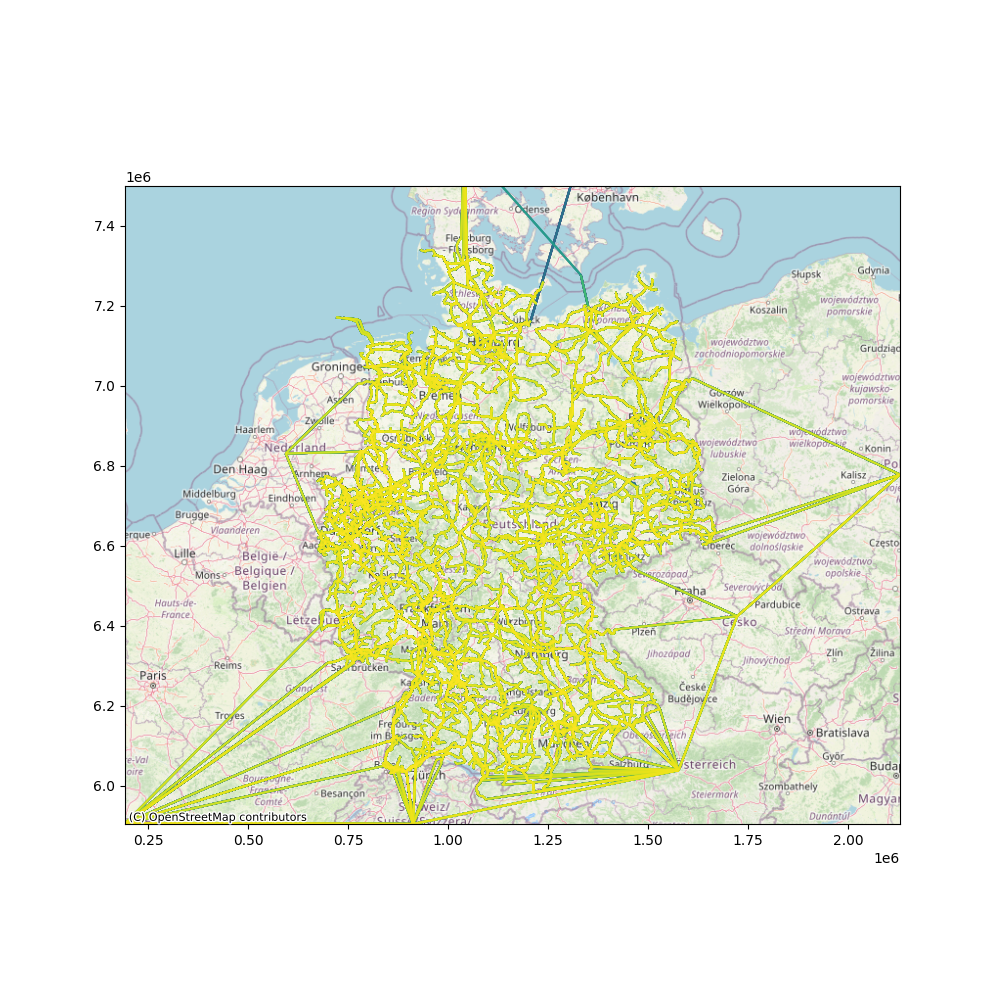
\includegraphics[width=.8\linewidth]{line.png}



\end{minipage}
\end{minipage}	
		
			
		
	\end{frame}


		%---------------------------------
	\begin{frame}
		\frametitle{Graphentheoretische Herangehensweise}
		\vspace*{2mm}
		\begin{minipage}{1\linewidth}
			\begin{minipage}{.4\linewidth}
				\vspace*{-8mm}
				Max-Flow-Min-Cut:
				\begin{itemize}
					
					\item Auswertung mit Zeitreihen
						\vspace*{2mm}
					
					\item Drei Produktions- und drei Verbraucherknoten
						\vspace*{2mm}
						
					\item um Max-Flow-Min-Cut anwenden zu können:
						\vspace*{2mm}
						\begin{itemize}
							\item [$\rightarrow$] jeweils einem gebündelten Knoten für In- und Output
							 
						\end{itemize}
					
					
					\vspace*{2mm}
					\item Problem: Einbezug von Verlust aktuell nicht möglich
									
					
				\end{itemize}
		
			\end{minipage}
			\hfill
			\begin{minipage}{.6\linewidth}
				\centering
				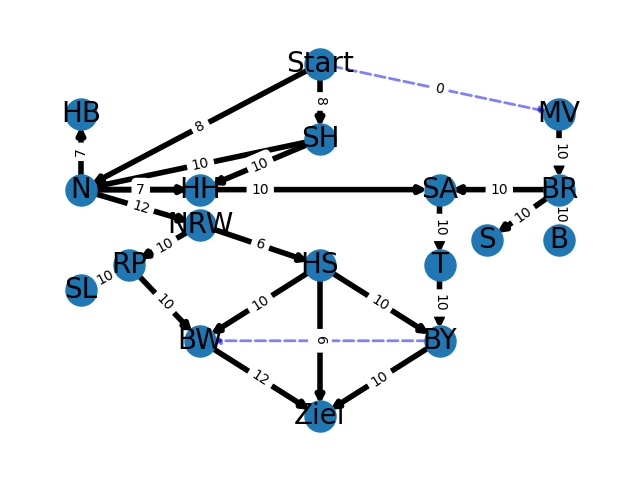
\includegraphics[width=.9\linewidth]{Figure_4.png}
				
			\end{minipage}
		\end{minipage}	
		
		
		
	\end{frame}
		%---------------------------------
	\begin{frame}
		\frametitle{}
		\vspace*{8mm}
		\begin{minipage}{1\linewidth}
		
			\begin{minipage}{.5\linewidth}
				\centering
				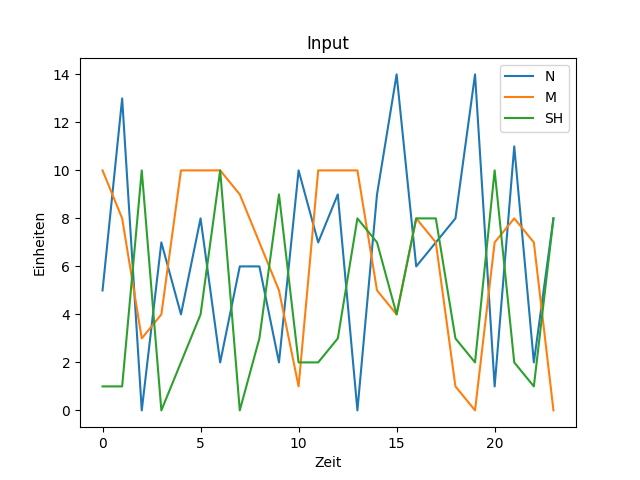
\includegraphics[width=1\linewidth]{Figure_1.png}
				
			\end{minipage}
			\hfill
			\begin{minipage}{.5\linewidth}
				\centering
				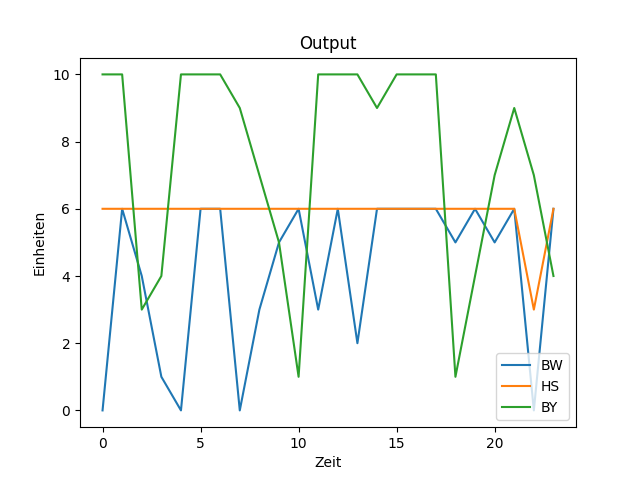
\includegraphics[width=1\linewidth]{Figure_2.png}
				
			\end{minipage}
		\end{minipage}	
		
		
		
	\end{frame}

		%---------------------------------
\begin{frame}
	\frametitle{}
	\vspace*{4mm}
	\begin{minipage}{0.9\linewidth}
		
		
			\centering
			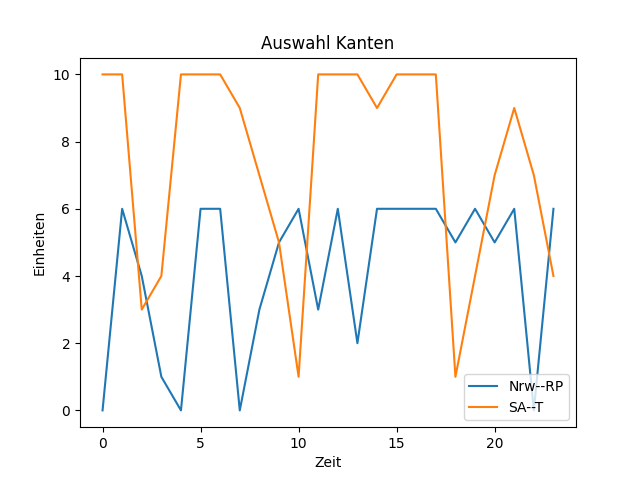
\includegraphics[width=0.6\linewidth]{Figure_3.png}
			
	\end{minipage}	
	
	
	
\end{frame}
	
	%---------------------------------
	
	\begin{frame}
		\frametitle{Modellierung}
		\vspace*{2mm}
		\begin{minipage}{1\linewidth}
			
				\begin{itemize}
					
					\item Betrachten von zwei Länder (Deutschland, Spanien)
					
					\item Daten: entsoe - Transperency Platform
					
					\item Länder haben Stromproduktion und -verbrauch
					
					\item bei Überproduktion Austausch von Strom möglich 
					
					\item Pipeline-Länge 2000km
					
					\item Baukosten Stromtrasse: 42 Mrd EUR (Anhand Beispiel SuedLink)
					
					\item 5\% Verlust pro 1000km (800 kV)
					
					\item Baukosten H2-Pipeline: 12,5 Mrd EUR (Anhand Beispiel Nord Stream)
					
					\item Verlust Umwandlung H2: 0.25 $\cdot$ 0.6
					
					\item Stromkosten Erneuerbar: $ 0.08 \frac{EUR}{kWh}$
					
					\item Stromkosten Konventionell: $ 0.8 \frac{EUR}{kWh}$
					
					\item Zeithorizont: 20 Jahre
					
				\end{itemize}
							
		
		\end{minipage}	
		
	\end{frame}


	%---------------------------------
	\begin{frame}
		\frametitle{Modell}
		\vspace{-2mm}
		
		
		\begin{minipage}{.9\linewidth}
			\centering
			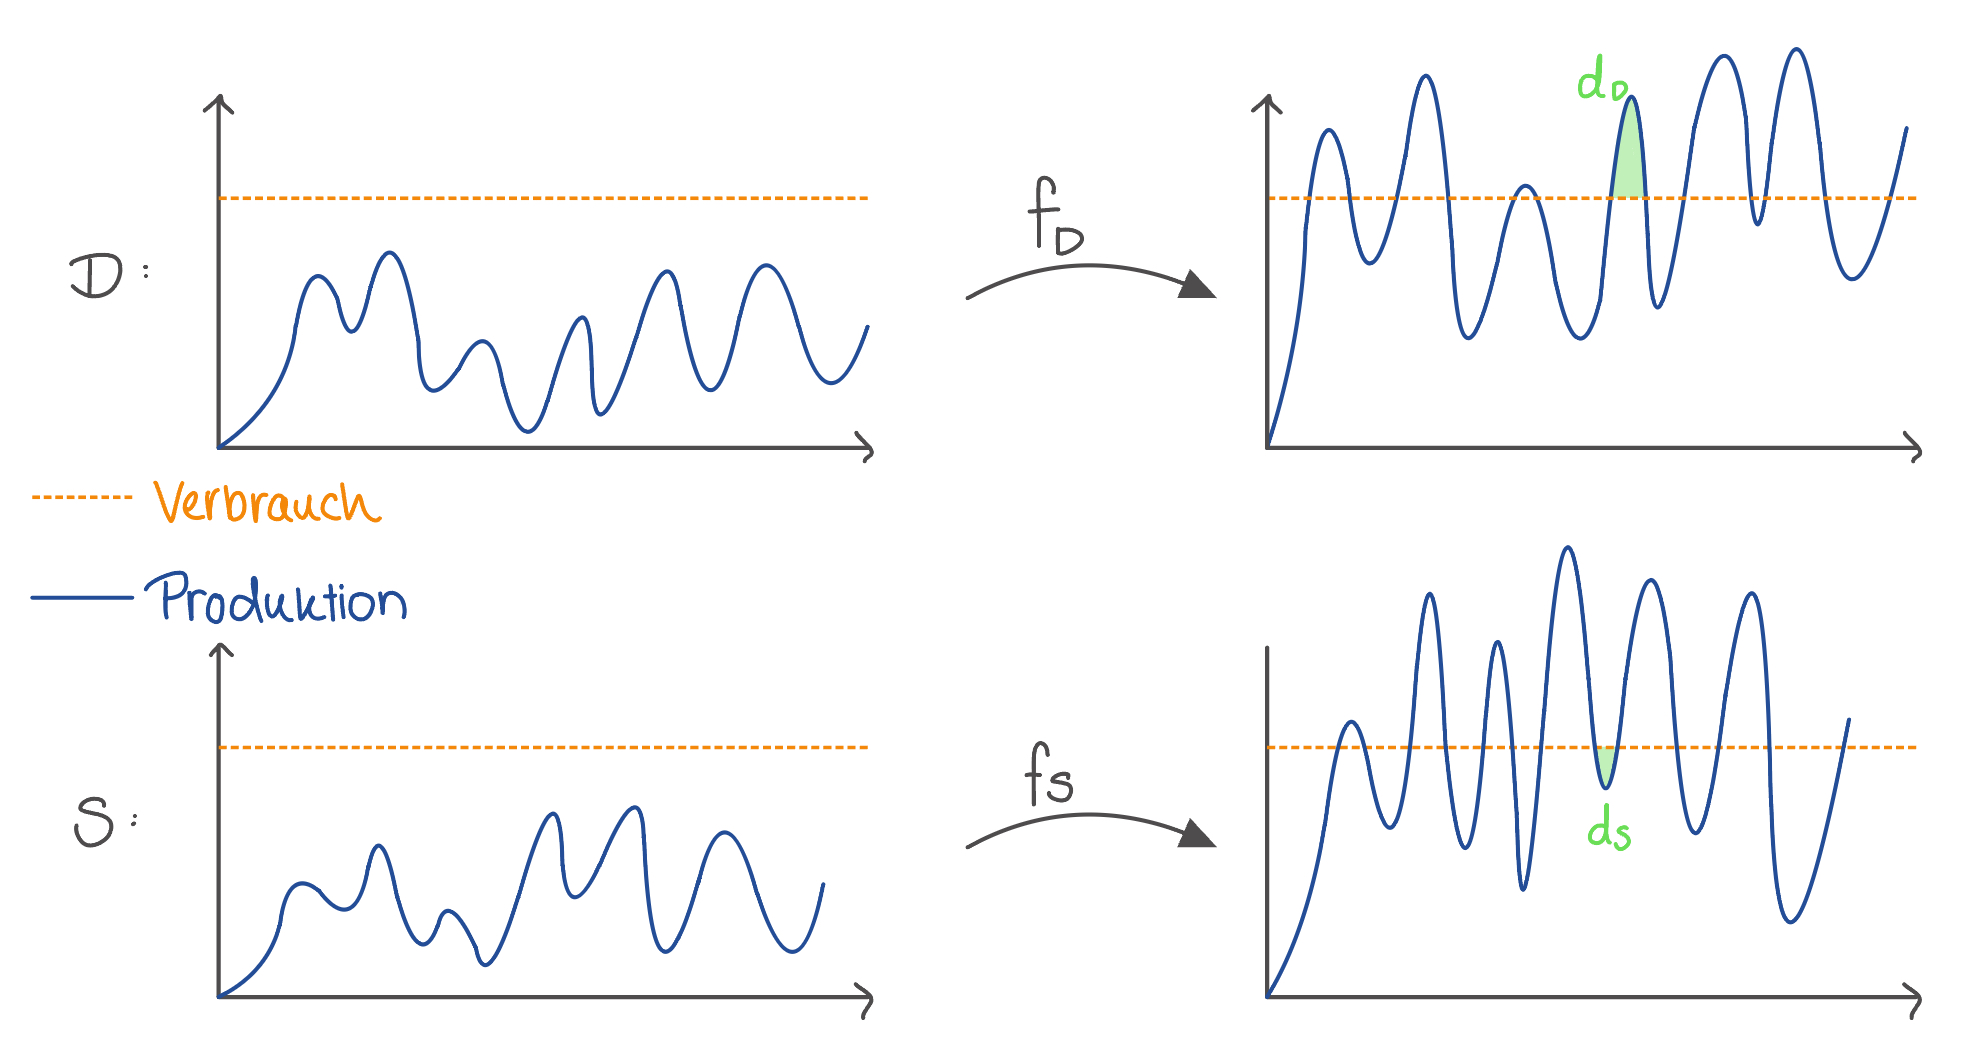
\includegraphics[width=.9\linewidth]{IMG_320.jpg}
			
		\end{minipage}
		
	\end{frame}


	%---------------------------------
	
	
	\begin{frame}
		\frametitle{Inputdaten I}
		\vspace{-2mm}
		\begin{figure}
			\includegraphics[width=0.6\linewidth]{de.pdf}
			\caption{Daten für Deutschland in MW, Skalierung von 100\%}
		\end{figure}
		
	\end{frame}
	
	\begin{frame}
		\frametitle{Inputdaten II}
		\vspace{-2mm}
		\begin{figure}
			\includegraphics[width=0.6\linewidth]{comparison.pdf}
			\caption{Nettoenergie in Deutschland und Spanien, Skalierung von 100\%}
		\end{figure}
	\end{frame}
	
	%---------------------------------
	\begin{frame}
		\frametitle{Kostenfunktion}
		\vspace*{2mm}
			\begin{minipage}{1\linewidth}
			\begin{minipage}{1\linewidth}
				\begin{itemize}
					\item \begin{math}
						J(f_D, f_S, c_{Strom}, c_{H2}) = (d_D + d_S) \cdot P_{Kohle} + P_{Leitung} \cdot c_{Strom} + P_{Erneuerbar}(f_D, f_S) + c_{H2} \cdot P_{H2}
					\end{math}
					\item 
					$	f_D$ = Skalierung der Produktion von Deutschland
					
					\item 
						$f_S$ = Skalierung der Produktion von Spanien
					\item 
					$	c$ = Kapazität
					\item 
					$	d$ = Differenz von Stromproduktion und  Stromverbrauch
				
					
				\end{itemize}
			\end{minipage}
			\hfill
			\begin{minipage}{.1\linewidth}
				\centering
				%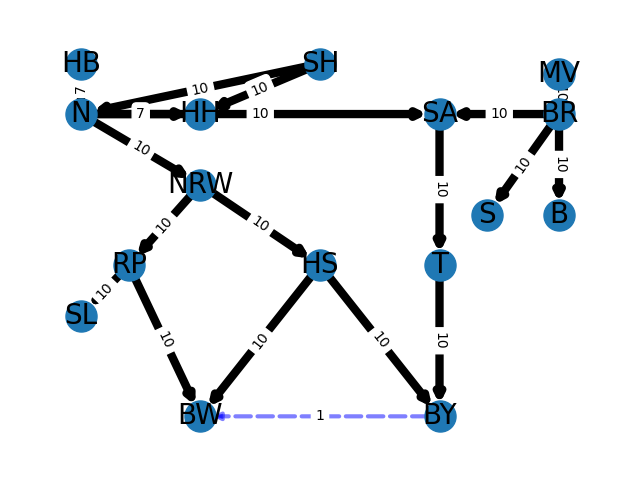
\includegraphics[width=.8\linewidth]{Example_graph_2.png}
				
			\end{minipage}
		\end{minipage}	
	
			
	\end{frame}

%---------------------------------

\begin{frame}
	\frametitle{Erste Ergebnisse I}
	\begin{itemize}
		\item Interessante Dynamik nur für (Straf-)Strompreis über 0.8 Euro
		\item Optimierung für alle vier Parameter gibt $f_D, f_S \geq 100\%$
		\item Kapazitäten sind in Summe bei über $3000$ MW
		\item Grafik für fixierte $f_D, f_S = 1.0$ auf folgender Seite
	\end{itemize}
	\vspace*{-2cm}
\end{frame}

\begin{frame}
	\frametitle{Erste Ergebnisse II}
	\vspace*{-1.6cm}
	% \hspace*{5cm}
	\begin{figure}
		\hspace*{3.5cm}\includegraphics[trim={3.4cm 1.0cm 3.4cm 1.0cm},clip, width=0.75\linewidth]{optimization.pdf}
		% \caption{Kostenfunktion für fixierte Skalierung der Renewables}
	\end{figure}x
\end{frame}



	%---------------------------------
	
	\begin{frame}
		\frametitle{Ausblick}
		Graphentheorie:
		\begin{itemize} 
			\item Automatisierung des Hinzufügen von Start- und Endknoten bei beliebigem Graph
			\item Verlust in Graphen einbinden
			\item Einbindung einer Zeitreihe für Verbrauch
			\item Graphentheoretischen Ansatz auf Modell anwenden
			
		\end{itemize}
		Modellierung:
		\begin{itemize}
			\item Erweiterung durch Hinzufügen von Ländern
			\item Erweiterung durch Speicherung von Wasserstoff
			\item Wird Verlust von Umwandlung von Strom-Wasserstoff-Strom sich verbessern?
			\item Eventuell Lastflussberechnung für Fantasie-Stromtrassen
		\end{itemize}
	\end{frame}
	
	


	%---------------------------------
	
	
	
	
	
	
\end{document}
% eof
